\documentclass{article}
\usepackage{amsmath}
\usepackage{diagbox}
\usepackage{enumitem}
\usepackage{pgfmath}
\usepackage{tikz}  % 引入TikZ包

\begin{document}

\section{2.9 Metric}
\subsection{(a)}
\begin{align}
(1)\rho(X,Y)&=H(X|Y)+H(Y|X)\\
         &\geq 0\\
(2)\rho(X,Y)&=\rho(Y,X)\\
(3)\rho(X,Y)+\rho(Y,Z)&=H(X|Y)+H(Y|X)+H(Y|Z)+H(Z|Y)\\
        &=H(X,Y)-H(Y)+H(X,Y)-H(X)+H(Y,Z)-H(Z)+H(Z,Y)-H(Y)\\
        &=2H(X,Y)+2H(Y,Z)-2H(Y)-H(X)-H(Z)\\
\rho(X,Z)&=H(X|Z)+H(Z|X)\\
         &=2H(X,Z)-H(Z)-H(X)\\
\Leftrightarrow \text{to show that:}\\
H(X,Y)+H(Y,Z)&\geq H(Y)+H(X,Z)\\
\text{we have:}\\
H(X,Y)+H(Y,Z)&=H(X,Y)+H(Z|Y)+H(Y)\\
             &\geq H(X,Y)+H(Z|X,Y)+H(Y)\\
             &H(X,Y,Z)+H(Y)\\
             &\geq H(X,Z)+H(Y).\\
\end{align}
\subsection{(b)}
\begin{align}
    \rho(X,Y)&=H(X|Y)+H(Y|X)\\
             &=2H(X,Y)-H(X)-H(Y)\\
    we~have~that:\\
       I(X,Y)&=H(X)+H(Y)-H(X,Y)\\
       \rho(X,Y)&=H(X,Y)-I(X,Y)\\
                &=H(X)+H(Y)-2I(X,Y).\\
\end{align}

\section{2.12 Example of joint entropy}
\begin{center}
\begin{tabular}{|c|c|c|}
\hline
\diagbox{$X$}{$Y$} & 0& 1 \\ \hline
0&1/3&1/3\\ \hline
1&0&1/3\\ \hline
\end{tabular}
\end{center}

\begin{itemize}
    \item 
    \begin{align}
    H(X)&=-(\frac{1}{3}log_2\frac{1}{3}+\frac{2}{3}log_2\frac{2}{3})\\
        &=log_2 3-\frac{2}{3}\\
    H(Y)&=-(\frac{1}{3}log_2\frac{1}{3}+\frac{2}{3}log_2\frac{2}{3})\\
        &=log_2 3-\frac{2}{3}\\
    \end{align}
    \item
    \begin{align}
    H(X|Y)&=-\sum_{y}p(x)H(X|Y=y)\\
          &=-(\frac{1}{3}H(X|Y=1)+\frac{2}{3}H(X|Y=0))\\
          &=-(\frac{1}{3}log_2\frac{1}{3})\\
          &=\frac{1}{3}log_2 3\\
    H(Y|X)&=-\sum_{x}p(x)H(Y|X=x)\\
          &=-(\frac{2}{3}H(Y|X=0)+\frac{1}{3}H(Y|X=1))\\
          &=-(\frac{2}{3}log_2\frac{2}{3})\\
          &=\frac{2}{3}log_2 3-\frac{2}{3}\\
    \end{align}
    \item  
    \begin{align}
    H(X,Y)&=H(X|Y)+H(Y)\\
          &=\frac{4}{3}log_2 3-\frac{2}{3}\\
    \end{align}
    \item 
    \begin{align}
    H(Y)-H(Y|X)&=\frac{1}{3}log_2 3\\
    \end{align}
    \item 
    \begin{align}
    H(X)-H(X|Y)&=H(Y)-H(Y|X)\\
               &=\frac{1}{3}log_2 3\\
    \end{align}
    \item Venn Diagram:
    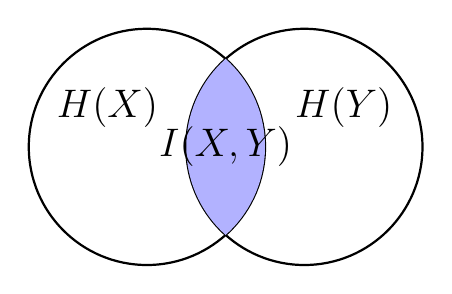
\begin{tikzpicture}
        % 画两个圆
        \draw[thick] (0,0) circle(1.5);  % A 集合
        \draw[thick] (2,0) circle(1.5);  % B 集合
        
        % 填充交集区域
        \begin{scope}
            \clip (0,0) circle(1.5);
            \clip (2,0) circle(1.5);
            \fill[blue!30] (-1.5,-1.5) rectangle (3.5,1.5);
        \end{scope}
        
        % 添加标签
        \node at (-0.5,0.5) {\Large $H(X)$};
        \node at (2.5,0.5) {\Large $H(Y)$};
        \node at (1,0) {\Large $I(X,Y)$}; % 交集部分
    \end{tikzpicture}
\end{itemize}

\section{2.35 Relative entropy is asymmetric}

\begin{center}
    \begin{tabular}{|c|c|c|}
    \hline
    Symbol&$p(x)$&$q(x)$\\ \hline
    a&$\frac{1}{2}$&$\frac{1}{3}$\\ \hline
    b&$\frac{1}{4}$&$\frac{1}{3}$\\ \hline
    c&$\frac{1}{4}$&$\frac{1}{3}$\\ \hline
    \end{tabular}
\end{center}
\begin{align}
H[p_x]&=H(\frac{1}{2},\frac{1}{4},\frac{1}{4})\\
      &=-(\frac{1}{2}\times(-1)+\frac{1}{4}\times(-2)+\frac{1}{4}\times(-2))\\
      &=\frac{3}{2}\\
H[q_x]&=H(\frac{1}{3},\frac{1}{3},\frac{1}{3})\\
      &=-3\times(\frac{1}{3}\times(log_2 \frac{1}{3}))\\
      &=log_2 3\\
D(p||q)&=\sum_{x\in X}p(x)log\frac{p(x)}{q(x)}\\
       &=\frac{1}{2}log_2\frac{3}{2}+\frac{1}{4}log_2\frac{3}{4}+\frac{1}{4}log_2\frac{3}{4}\\
       &=log_2 3-\frac{3}{2}
D(q||p)&=\sum_{x\in X}q(x)log\frac{q(x)}{p(x)}\\
       &=\frac{1}{3}log_2\frac{2}{3}+\frac{2}{3}log_2\frac{4}{3}\\
       &=\frac{1}{3}log_2\frac{8}{9}\\
       &\frac{5}{3}-log_2 3\\
D(q||p)\neq D(p||q).
\end{align}

\section{2.43 Mutual information of heads and tails}
\subsection{(a)}
Let the random variable $X\sim B(\frac{1}{2})$,$Y=1-X$.

\begin{center}
    \begin{tabular}{c|c|c}
    \hline
    \diagbox{$X$}{$Y$} & 0& 1 \\ \hline
    0&0&$\frac{1}{2}$\\ \hline
    1&$\frac{1}{2}$&0\\ \hline
    \end{tabular}
\end{center}
\begin{align}
H(X|Y)&=0\\
I(X,Y)&=H(X)-H(X|Y)\\
      &=H(\frac{1}{2},\frac{1}{2})-0\\
      &=1 bit    
\end{align}

\subsection{(b)}
Let the random variable $X,Y$ be two sides, then:
\begin{align}
p(X)&=p(Y)=\frac{1}{6}\\
H(X)&=H(Y)=-\frac{1}{6}\sum_{1}^{6}log_2\frac{1}{6}\\
    &=log_2 6\\
p(X,Y)&=\frac{1}{\binom{6}{2}}\\
      &=\frac{1}{24}\\
H(X,Y)&=-\sum_{x,y}p(x,y)log_2p(x,y)\\
      &=log_2 24\\
I(X,Y)&=H(X)+H(Y)-H(X,Y)\\
      &=2log_2 6-log_2 24\\
      &=log_2\frac{3}{2}\\
      &\approx 0.585 bit
\end{align}

\end{document}
